\section{GPU 和 GPU 芯片}

\subsection{GPU芯片的定义}

本章我们将比较两个关键术语：GPU 和 GPU 芯片。本章非常重要，因为如果不理解 GPU 与 GPU 芯片之间的区别，就无法解释英伟
达生产的各种架构。

首先来说明这两个术语的区别，从 GPU 芯片开始。GPU 芯片代表着 GPU 的心脏——它是实际的硅核心，不附带任何外围组件。例如
，一款名为 GF100 的 GPU 芯片，其中的 F 指 Fermi 架构。在该芯片内部，集成了各种核心、内存控制器和其他负责 GPU 计算的电
子元件。而 GPU 则是消费者购买的最终产品，它集成了芯片以及必要的系统和接口，包括许多 GPU 中都存在的冷却机制。

\begin{figure}
    \centering
    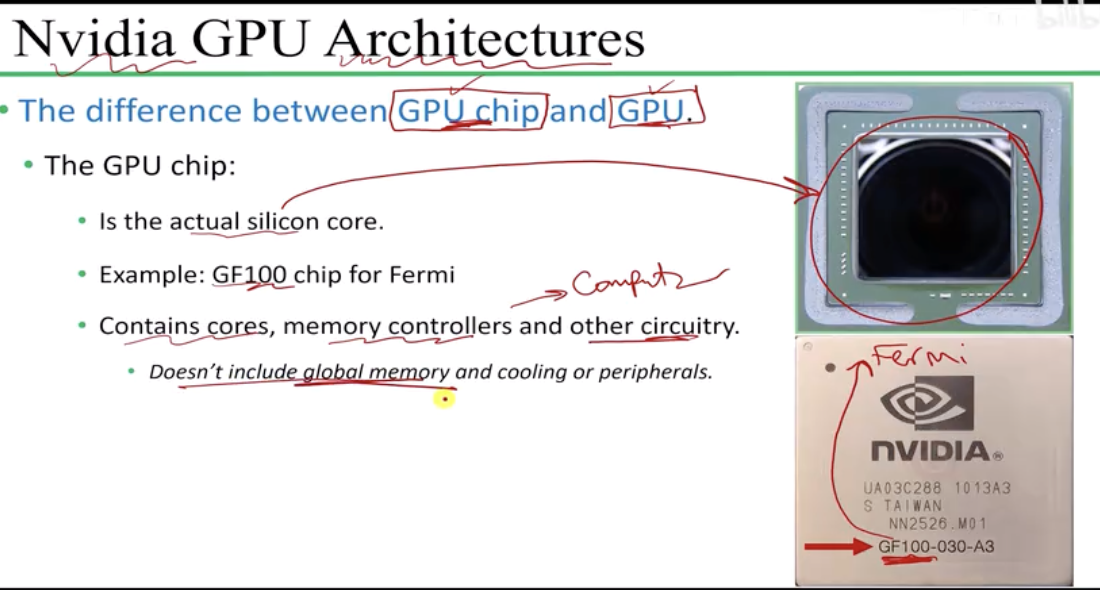
\includegraphics[width=0.75\linewidth]{resources/cuda-017.png}
    \caption{GPU 和 GPU 芯片}
    \label{fig:placeholder}
\end{figure}


\subsection{GeForce GTX 480与GF100芯片}

这款 GPU 由上文讨论过的 GF100 芯片驱动。下图展示的是 GeForce GTX 480 GPU——除了 GF100 芯片之外，它还包含全局内存单
元、显示端口（如 HDMI 端口）和一个冷却风扇。之所以需要冷却风扇，是因为它属于 GeForce 世代，这类环境需要风扇来散发计算
产生的热量。

\begin{figure}
    \centering
    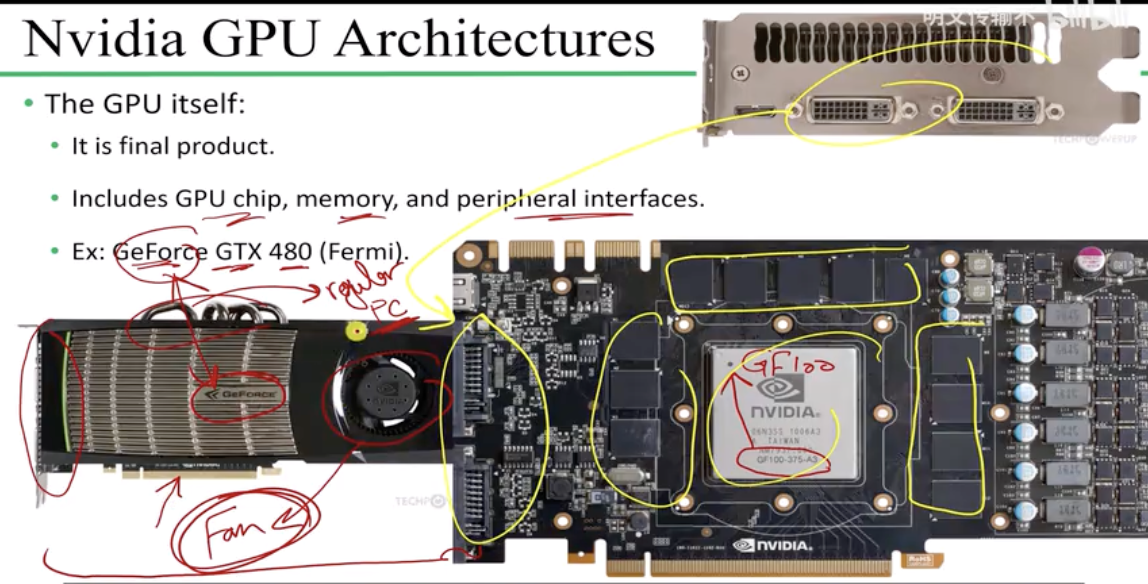
\includegraphics[width=0.75\linewidth]{resources/cuda-018.png}
    \caption{GPU 和 GPU 芯片}
    \label{fig:placeholder}
\end{figure}

根据之前的讨论，GeForce 世代是面向普通消费者的标准台式机和工作站设计的。

\subsection{A100与GA100芯片}

这两个术语之间区别的另一个例子可以从 A100 GPU 及其芯片中看到。基于 Ampere 架构的 A100 GPU，其名称中的字母 A 即体现
了这一点。与 Fermi 芯片类似的命名方式，驱动 A100 GPU 的芯片为 GA100。

\begin{figure}
    \centering
    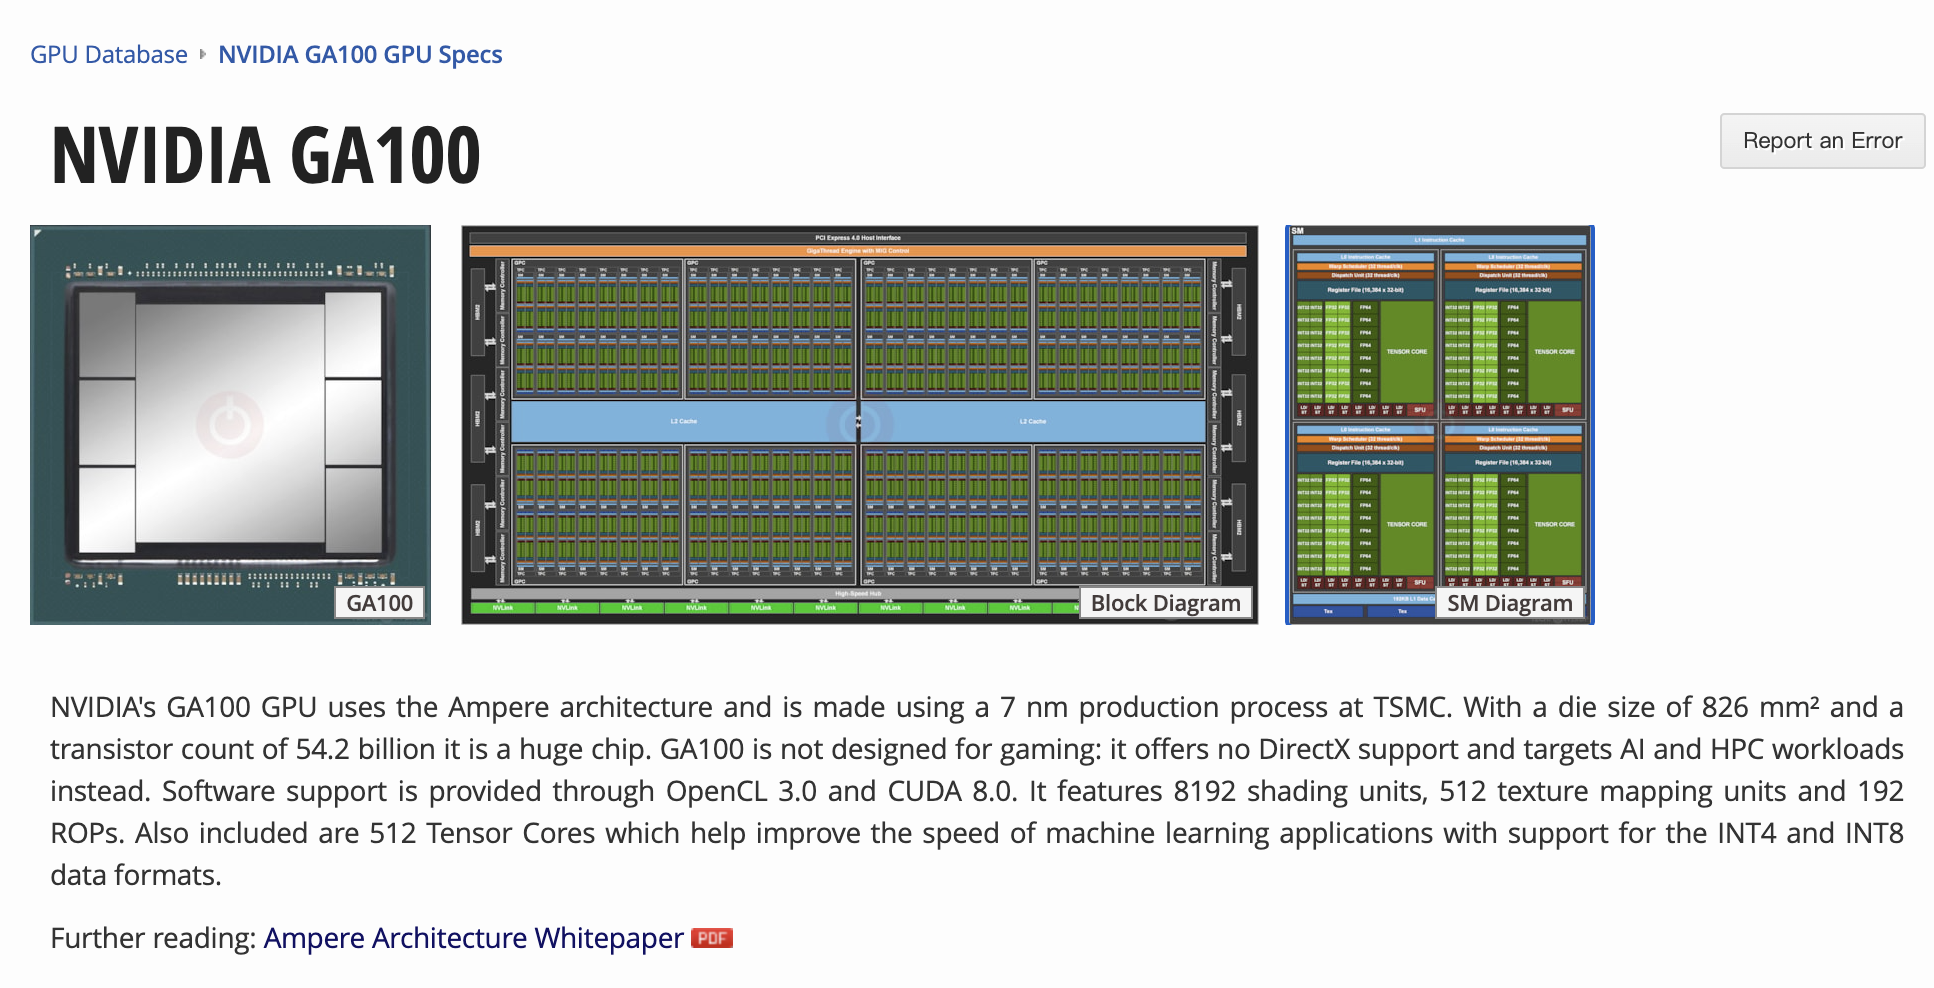
\includegraphics[width=0.75\linewidth]{resources/cuda-019.png}
    \caption{GA100芯片}
    \label{fig:placeholder}
\end{figure}

在 Fermi 架构中，芯片命名为 GF100。在 Ampere 架构中，芯片命名为 GA100。访问 TechPowerUp 网站，可以看到 A100 GPU 
的众多规格，网页上首先展示的就是芯片名称——GA100。通过搜索芯片名称 GA100，可以找到对应的链接，点击即可看到 GA100
芯片：如图所示，它仅是一块电子芯片，没有连接任何其他组件。

回到 A100 GPU 的网页，可以看到 A100 GPU 包含芯片、内存单元和其他外围组件。总而言之，GPU 芯片是 GPU 的核心，而 GPU 
本身是包含芯片、内存接口和冷却系统的完整产品，可以直接供消费者使用。
